\documentclass[11pt]{beamer}
% \usetheme{Boadilla}
  \usetheme{default}


% acronyms for text or math mode
\newcommand {\ccast} {\mbox{\small CCAST}}
\newcommand {\cris} {\mbox{\small CrIS}}

\newcommand {\airs} {\mbox{\small AIRS}}
\newcommand {\iasi} {\mbox{\small IASI}}
\newcommand {\idps} {\mbox{\small IDPS}}
\newcommand {\nasa} {\mbox{\small NASA}}
\newcommand {\noaa} {\mbox{\small NOAA}}
\newcommand {\nstar} {\mbox{\small STAR}}
\newcommand {\umbc} {\mbox{\small UMBC}}
\newcommand {\uw}   {\mbox{\small UW}}

\newcommand {\fft}  {\mbox{\small FFT}}
\newcommand {\ifft} {\mbox{\small IFFT}}
\newcommand {\fir}  {\mbox{\small FIR}}
\newcommand {\fov}  {\mbox{\small FOV}}
\newcommand {\for}  {\mbox{\small FOR}}
\newcommand {\ict}  {\mbox{\small ICT}}
\newcommand {\ils}  {\mbox{\small ILS}}
\newcommand {\igm}  {\mbox{\small IGM}}
\newcommand {\opd}  {\mbox{\small OPD}}
\newcommand {\rms}  {\mbox{\small RMS}}
\newcommand {\zpd}  {\mbox{\small ZPD}}
\newcommand {\ppm}  {\mbox{\small PPM}}
\newcommand {\srf}  {\mbox{\small SRF}}
\newcommand {\sdr}  {\mbox{\small SDR}}

\newcommand {\ES} {\mbox{\small ES}}
\newcommand {\SP} {\mbox{\small SP}}
\newcommand {\IT} {\mbox{\small IT}}
\newcommand {\SA} {\mbox{\small SA}}

\newcommand {\ET} {\mbox{\small ET}}
\newcommand {\FT} {\mbox{\small FT}}

% abbreviations, mainly for math mode
\newcommand {\real} {\mbox{real}}
\newcommand {\imag} {\mbox{imag}}
\newcommand {\atan} {\mbox{atan}}
\newcommand {\obs}  {\mbox{obs}}
\newcommand {\calc} {\mbox{calc}}
\newcommand {\sinc} {\mbox{sinc}}
\newcommand {\psinc} {\mbox{psinc}}
\newcommand {\std} {\mbox{std}}

% symbols, for math mode only
\newcommand {\wnum} {\mbox{cm$^{-1}$}}
\newcommand {\lmax} {L_{\mbox{\tiny max}}}
\newcommand {\vmax} {V_{\mbox{\tiny max}}}

\newcommand {\tauobs} {\tau_{\mbox{\tiny obs}}}
\newcommand {\taucal} {\tau_{\mbox{\tiny calc}}}
\newcommand {\Vdc}  {V_{\mbox{\tiny DC}}}

\newcommand {\rIT} {r_{\mbox{\tiny\textsc{ict}}}}
\newcommand {\rES} {r_{\mbox{\tiny\textsc{es}}}}
\newcommand {\robs} {r_{\mbox{\tiny obs}}}

\newcommand {\rITobs} {r_{\mbox{\tiny\textsc{ict}}}^{\mbox{\tiny obs}}}
\newcommand {\rITcal} {r_{\mbox{\tiny\textsc{ict}}}^{\mbox{\tiny cal}}}

\newcommand {\ITmean} {\langle\mbox{\small IT}\rangle}
\newcommand {\SPmean} {\langle\mbox{\small SP}\rangle}


\title{Standard and periodic sinc ILS \\
  for the CrIS high resolution tests}
\author{H.~E.~Motteler and L.~L.~Strow}
\institute{
  UMBC Atmospheric Spectroscopy Lab \\
  Joint Center for Earth Systems Technology \\
}
\date{\today}
\begin{document}

%----------- slide --------------------------------------------------%
\begin{frame}[plain]
\titlepage
\end{frame}
%----------- slide --------------------------------------------------%
\begin{frame}
\frametitle{abstract}

Using data from the 2013 high res tests, a comparison of FOV means
for the SW band shows a significant reduction in variation with periodic
sinc as the ILS basis function.  The periodic sinc ILS also gives a
significant reduction in obs minus calc for a clear subset from the
27--28 Aug 2013 tests that we made available earlier.

\hspace{4cm}

Thanks to Dan Mooney for the derivation of the periodic sinc ILS
basis, and for his advice in applying those derivations.

\end{frame}
%----------- slide --------------------------------------------------%
\begin{frame}
\frametitle{test design}

\begin{itemize}
  \item we take the average of each FOV over the high res test for
    FOR 15 and 16 ascending, and compare these with the average for
    FOV 5

  \item to the extent that different FOV views dissappear in the
    averages, this can reveal differences in detector response or
    FOV-related problems with modeling or processing

  \item we also look at the standard deviation of each FOV over the
    high res test, and compare these with the standard deviation for
    FOV 5

  \item for the obs minus calc, we start with a clear subset of
    around 100 profiles from the Aug 2013 high res test, and
    calculate expected upwelling radiances

  \item in addition to simple obs minus calc, we compare biases with
    and without Hamming apodization

\end{itemize}

\end{frame}
%----------- slide --------------------------------------------------%
\begin{frame}
\frametitle{sinc and psinc ils}

\begin{center}
  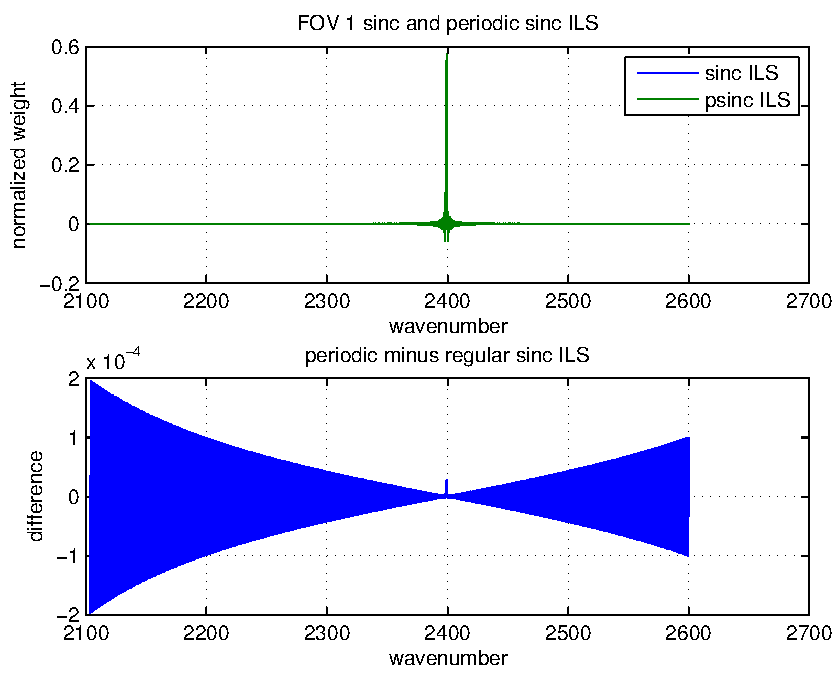
\includegraphics[scale=0.6]{figures/psinc_demo.pdf}
\end{center}

sensor grid regular and periodic sinc ILS functions

\end{frame}
%----------- slide --------------------------------------------------%
\begin{frame}
\frametitle{sinc fov means}

\begin{center}
  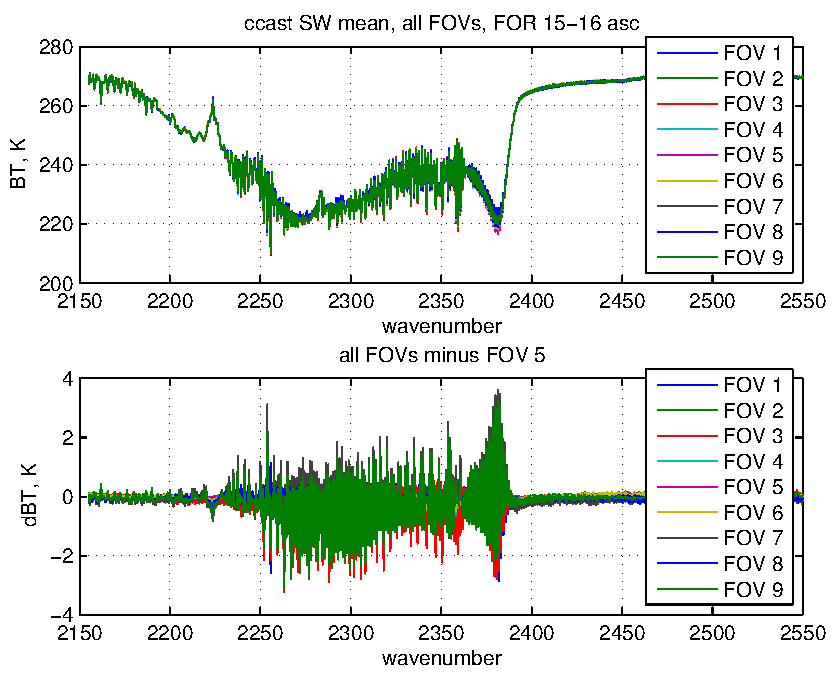
\includegraphics[scale=0.6]{figures/hr2_avg_s.pdf}
\end{center}

FOV means and differences from FOV 5, for the regular sinc ILS

\end{frame}
%----------- slide --------------------------------------------------%
\begin{frame}
\frametitle{psinc fov means}

\begin{center}
  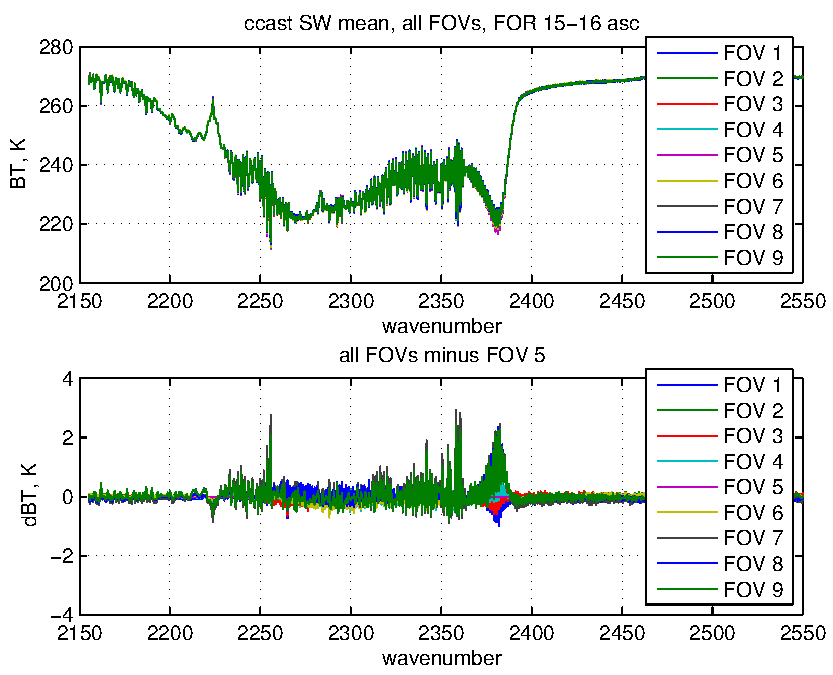
\includegraphics[scale=0.6]{figures/hr2_avg_p.pdf}
\end{center}

FOV means and differences from FOV 5, for the periodic sinc ILS

\end{frame}
%----------- slide --------------------------------------------------%
\begin{frame}
\frametitle{sinc breakout}

\begin{center}
  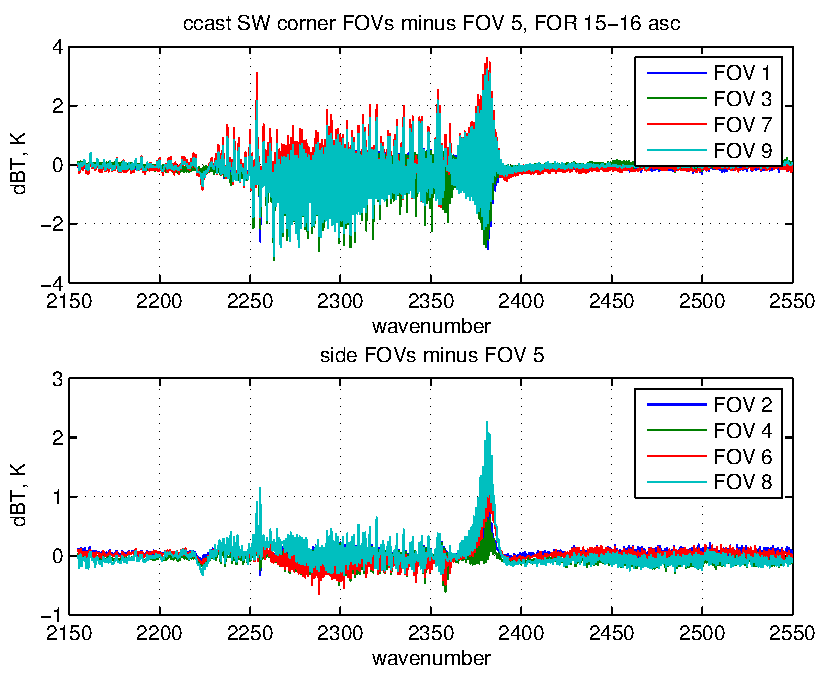
\includegraphics[scale=0.6]{figures/hr2_dif_s.pdf}
\end{center}

breakout of mean differences for the regular sinc ILS

\end{frame}
%----------- slide --------------------------------------------------%
\begin{frame}
\frametitle{psinc breakout}

\begin{center}
  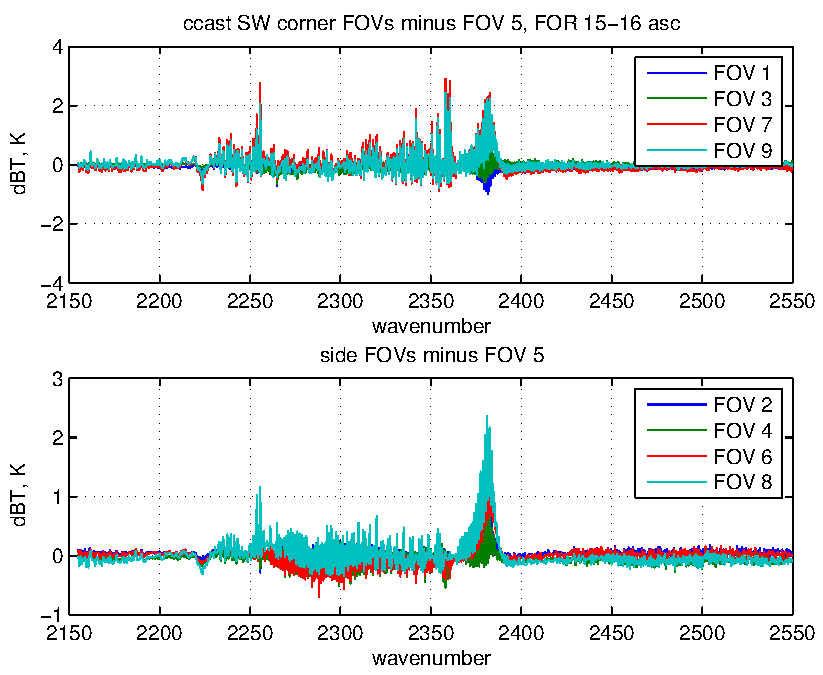
\includegraphics[scale=0.6]{figures/hr2_dif_p.pdf}
\end{center}

breakout of mean differences for the periodic sinc ILS

\end{frame}
%----------- slide --------------------------------------------------%
\begin{frame}
\frametitle{sinc fov stds}

\begin{center}
  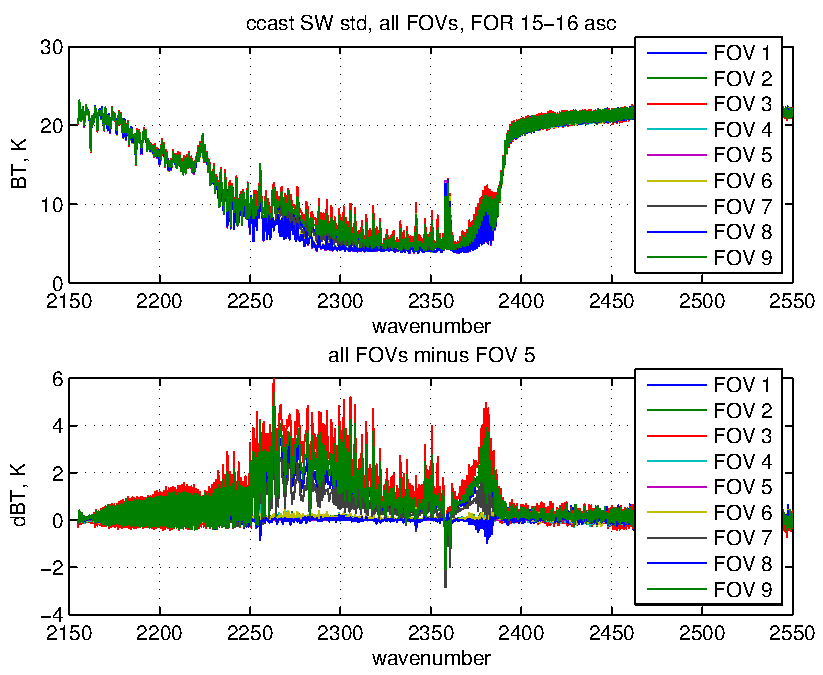
\includegraphics[scale=0.6]{figures/hr2_std_s.pdf}
\end{center}

FOV standard deviations and the differences of the standard
deviations from FOV 5, for the regular sinc ILS

\end{frame}
%----------- slide --------------------------------------------------%
\begin{frame}
\frametitle{psinc fov stds}

\begin{center}
  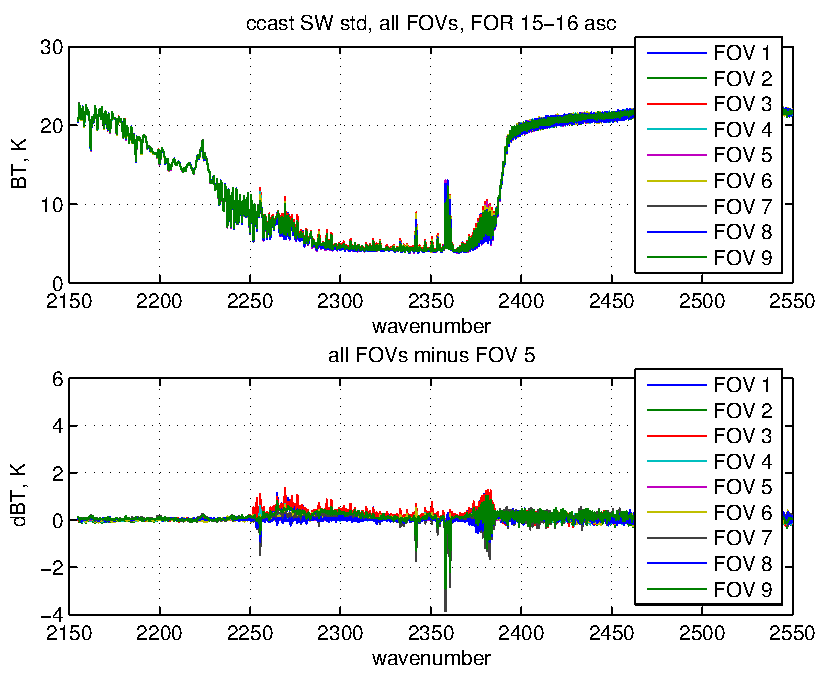
\includegraphics[scale=0.6]{figures/hr2_std_p.pdf}
\end{center}

FOV standard deviations and the differences of the standard
deviations from FOV 5, for the periodic sinc ILS

\end{frame}
%----------- slide --(old #6)----------------------------------------%
\begin{frame}
\frametitle{obs minus calc}

\begin{center}
  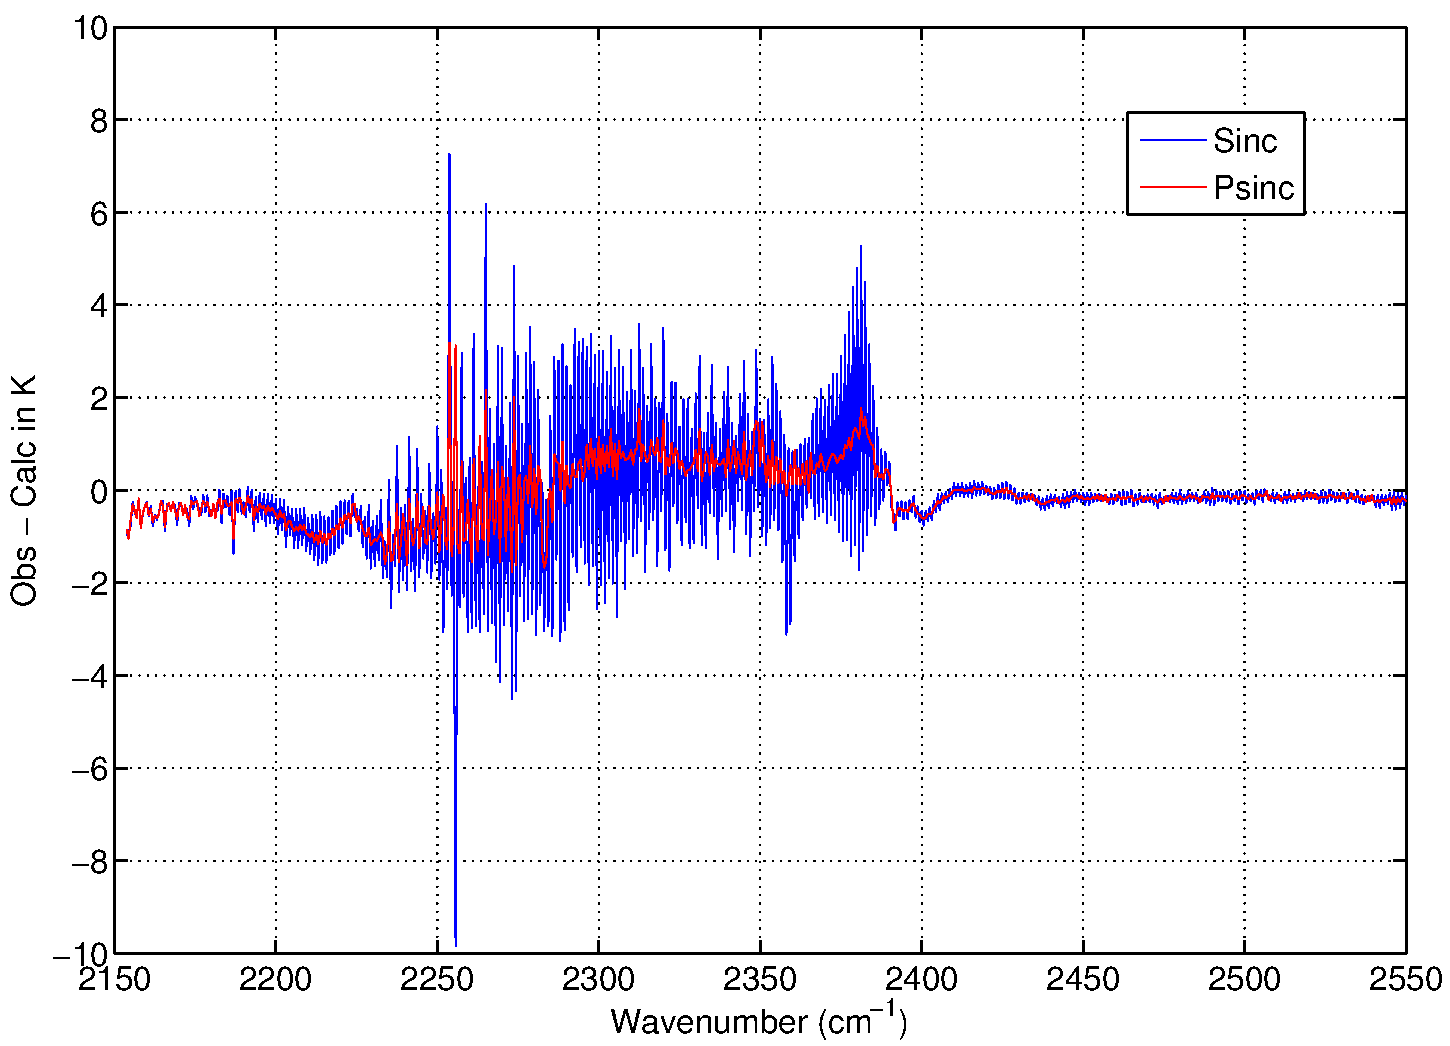
\includegraphics[scale=0.4]{strow_figs/bias_sinc_shortwave.pdf}
\end{center}

clear subset $\obs - \calc$ brightness temps, for sinc and psinc

\end{frame}
%----------- slide --(old #1)----------------------------------------%
\begin{frame}
\frametitle{hamming obs minus calc}

\begin{center}
  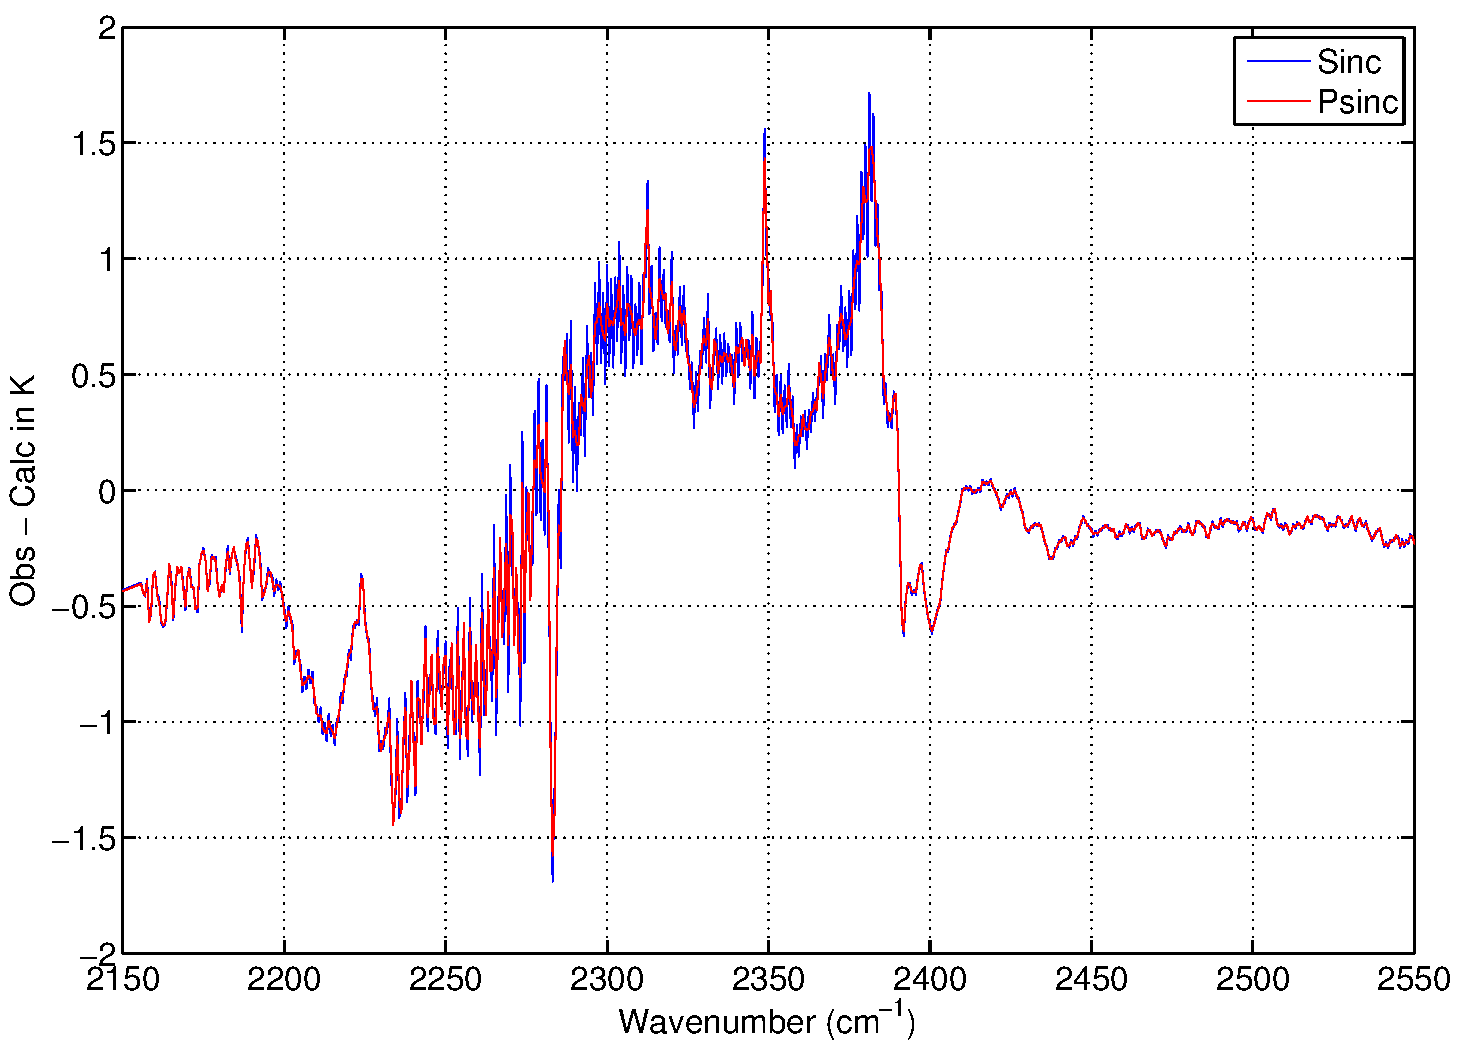
\includegraphics[scale=0.4]{strow_figs/bias_ham_shortwave.pdf}
\end{center}

clear subset $H(\obs) - H(\calc)$ BT.  $H$ is Hamming apodization.

\end{frame}
%----------- slide --(old #5)----------------------------------------%
\begin{frame}
\frametitle{residual comparison}

\begin{center}
  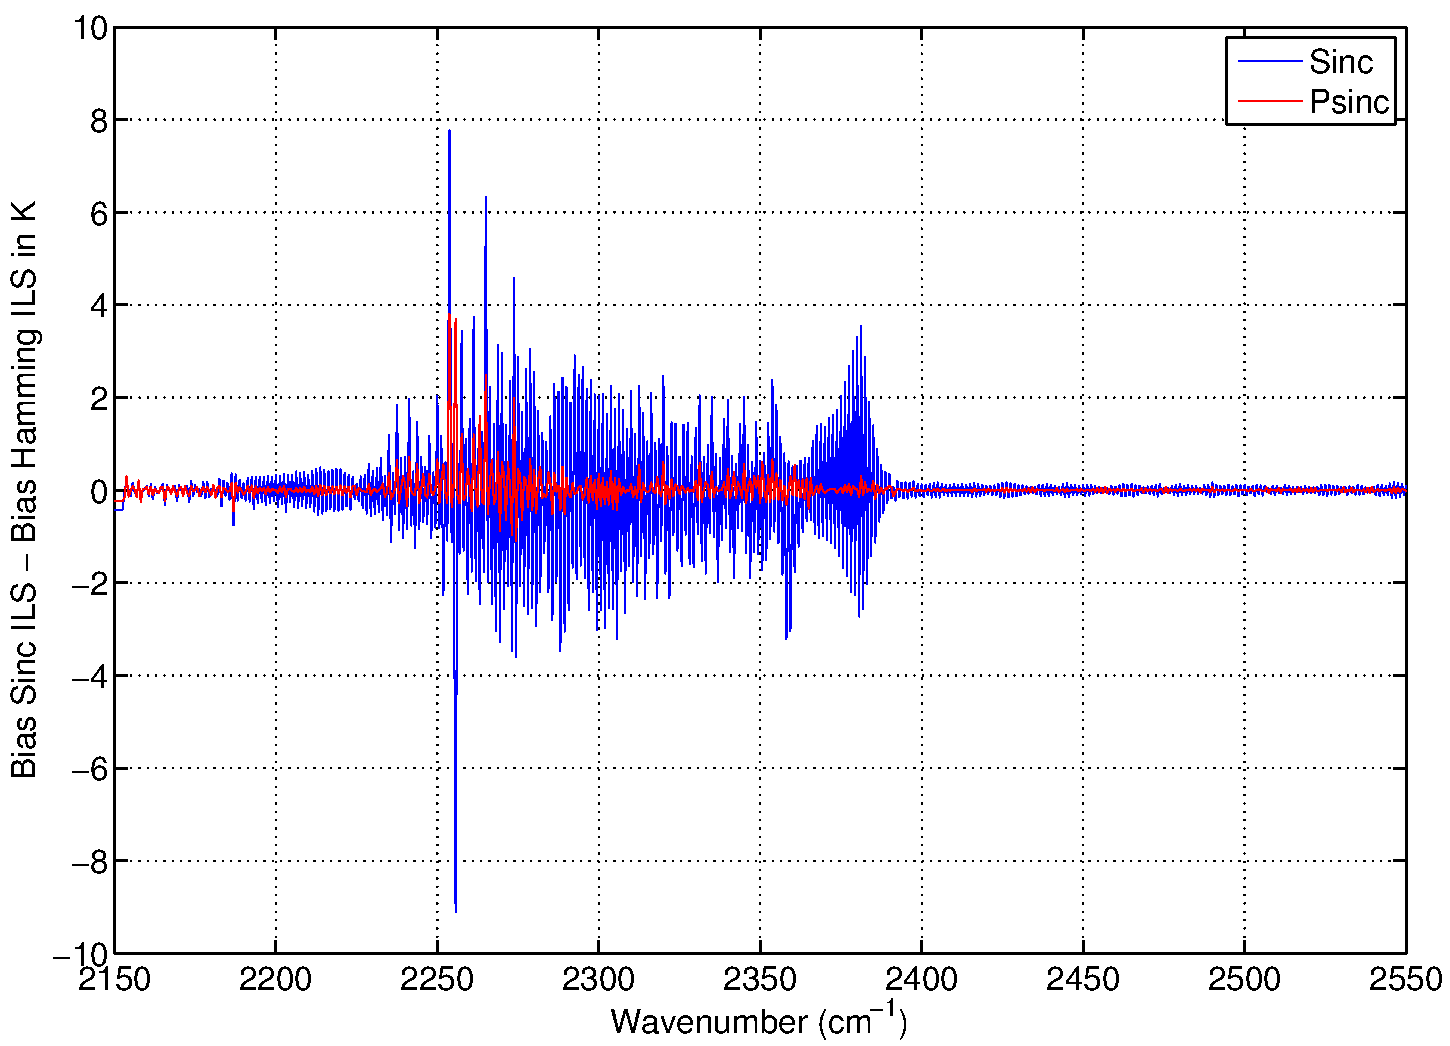
\includegraphics[scale=0.4]{strow_figs/bias_sinc_minus_bias_ham.pdf}
\end{center}

clear subset $(\obs - \calc) - (H(\obs) - H(\calc))$ BT

\end{frame}
%----------- slide --(old #7)----------------------------------------%
\begin{frame}
\frametitle{radiance obs and calc}

\begin{center}
  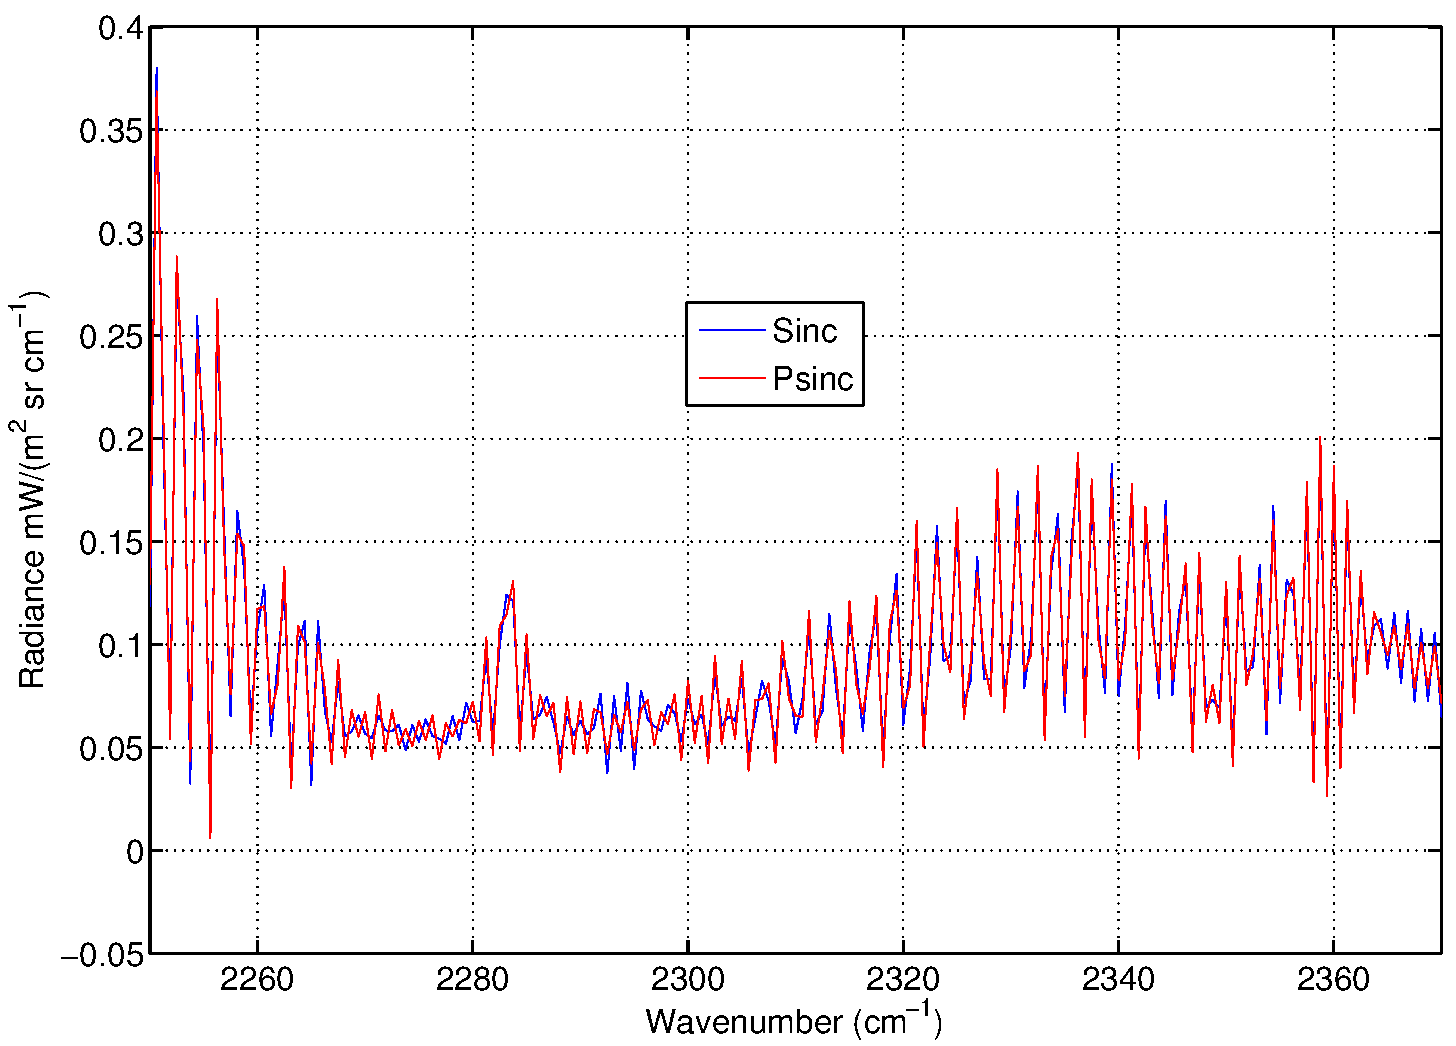
\includegraphics[scale=0.4]{strow_figs/sinc_vs_psinc_rad_sw.pdf}
\end{center}

clear subset zoom of radiance obs and calc 

\end{frame}
%----------- slide --------------------------------------------------%
\begin{frame}
\frametitle{conclusions}

\begin{itemize}
  \item we see significant reductions in the variation of FOV
    response and in observed and calculated residuals with the
    periodic sinc for the Aug 2013 high res tests

  \item we saw a similar significant reduction in the variation of
    FOV response with the periodic sinc for the March 2013 high res
    tests

  \item analyzing data from the gas cell bench tests last fall, we
    did not see an improvement using periodic sinc for the LW CO$_2$
    tests.  But there are hints of it here, shown in the supporting
    slides.
    
  \item all processing and tests were done with ccast, changing a
    couple of lines of code to switch from regular to periodic sinc

\end{itemize}

\end{frame}
%----------- slide --(old #2)---------------------------------------%
\begin{frame}
\frametitle{obs minus calc}

\begin{center}
  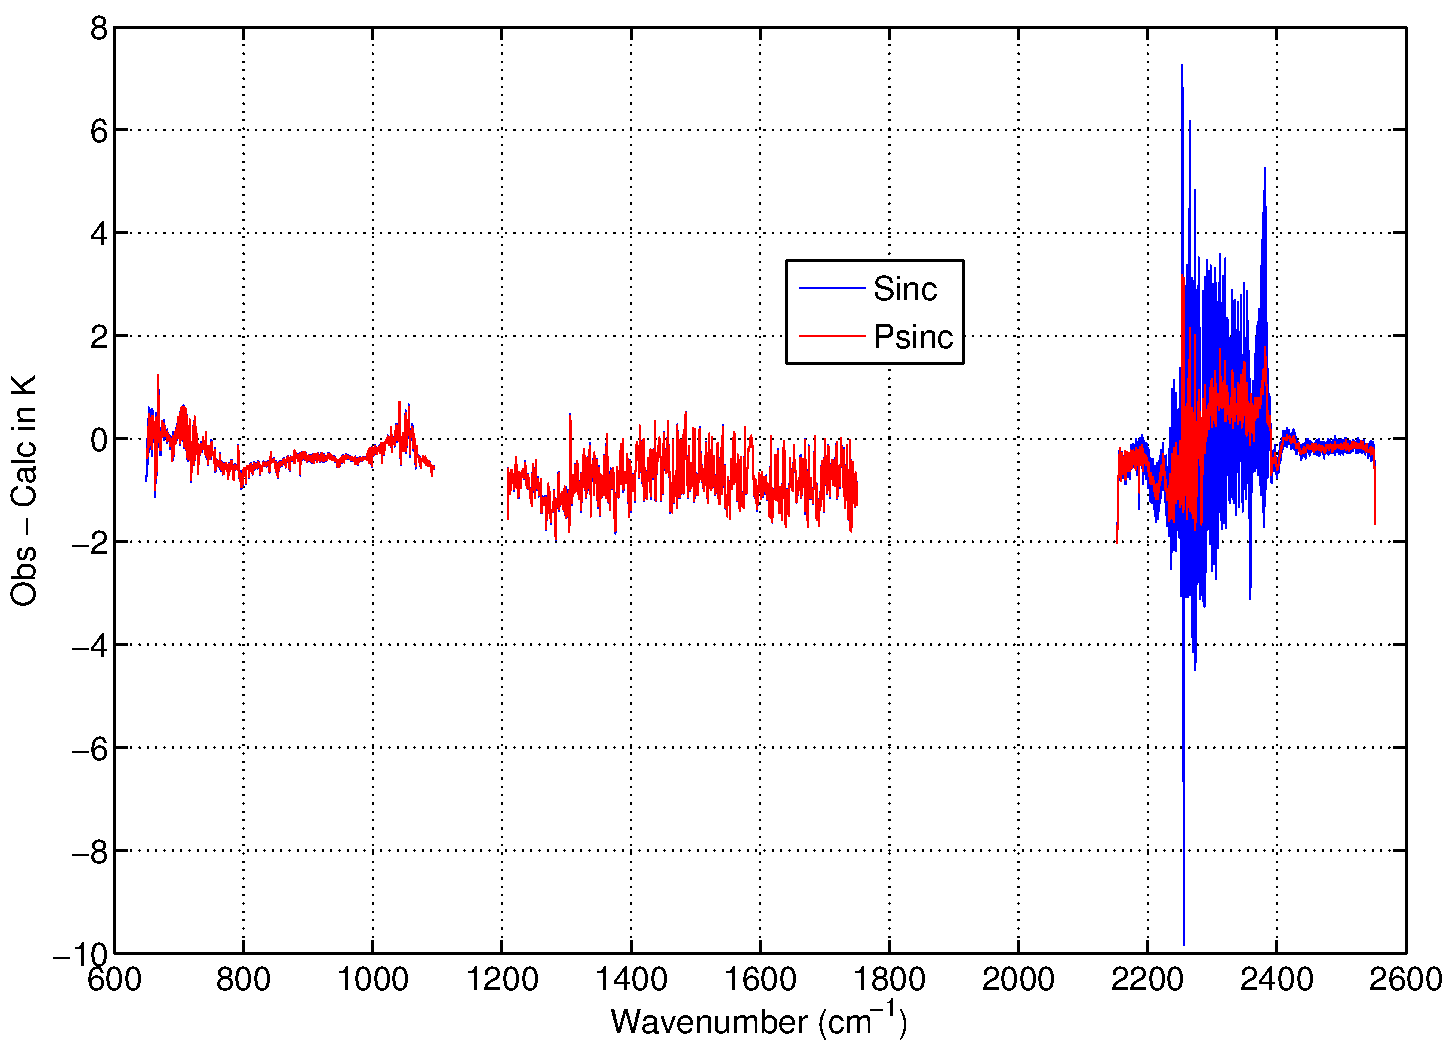
\includegraphics[scale=0.4]{strow_figs/bias_sinc_allnu.pdf}
\end{center}

all bands $\obs - \calc$ BT

\end{frame}
%----------- slide --(old #3)----------------------------------------%
\begin{frame}
\frametitle{obs minus calc zoom}

\begin{center}
  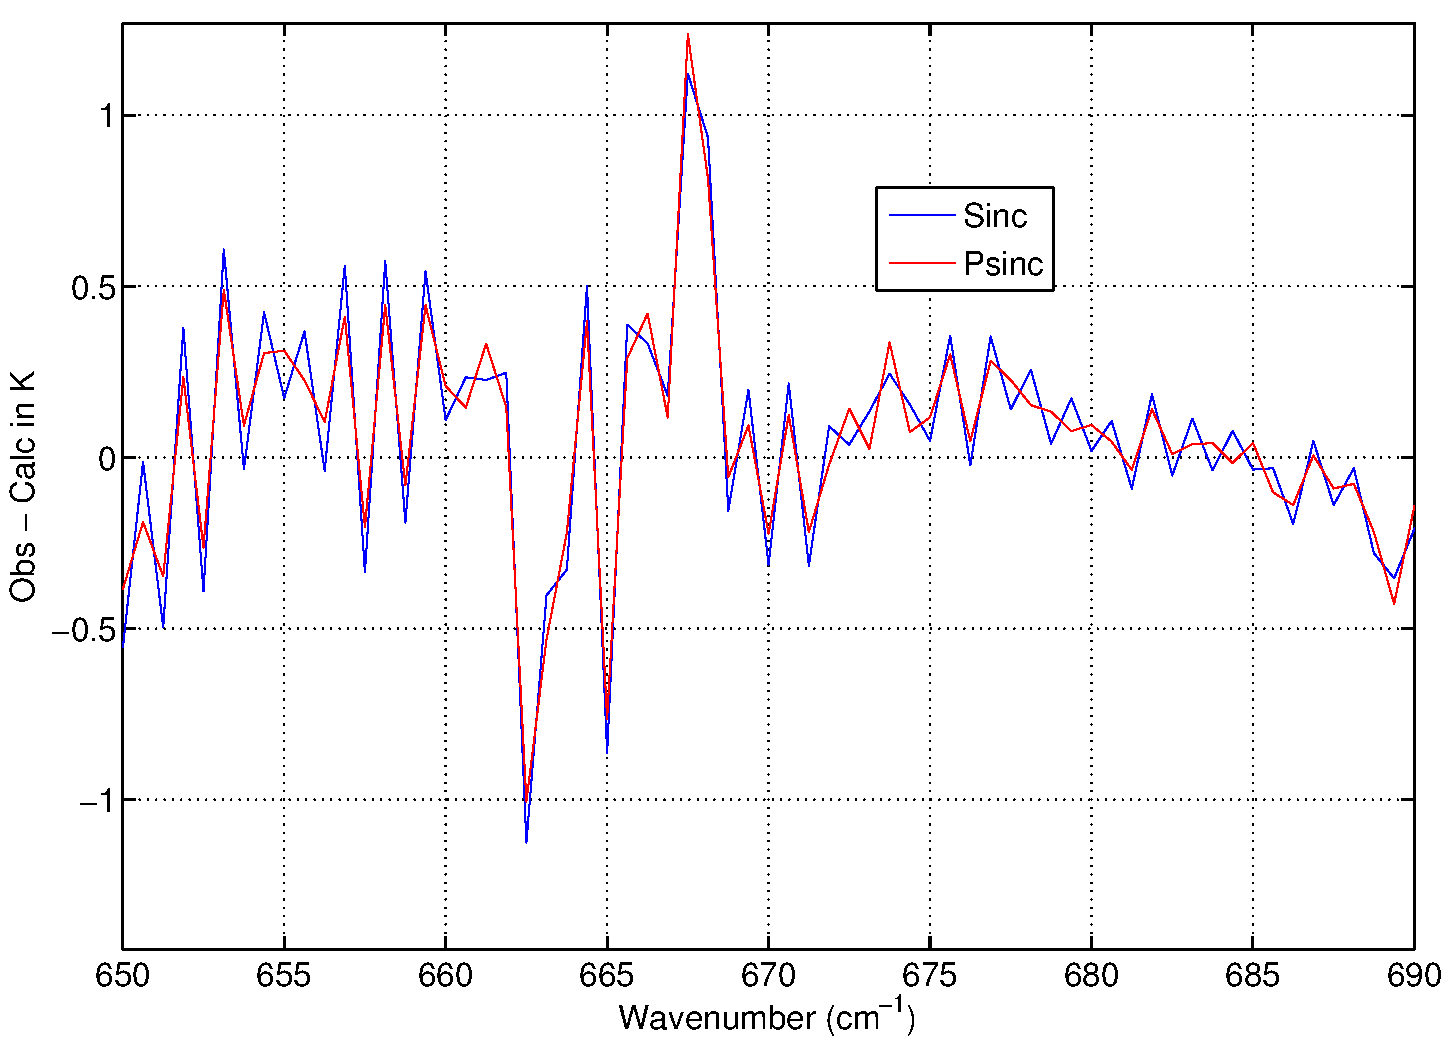
\includegraphics[scale=0.4]{strow_figs/bias_sinc_longwave.pdf}
\end{center}

LW zoom of  $\obs - \calc$ BT

\end{frame}
%----------- slide --(old #4)----------------------------------------%
\begin{frame}
\frametitle{residual comparison}

\begin{center}
  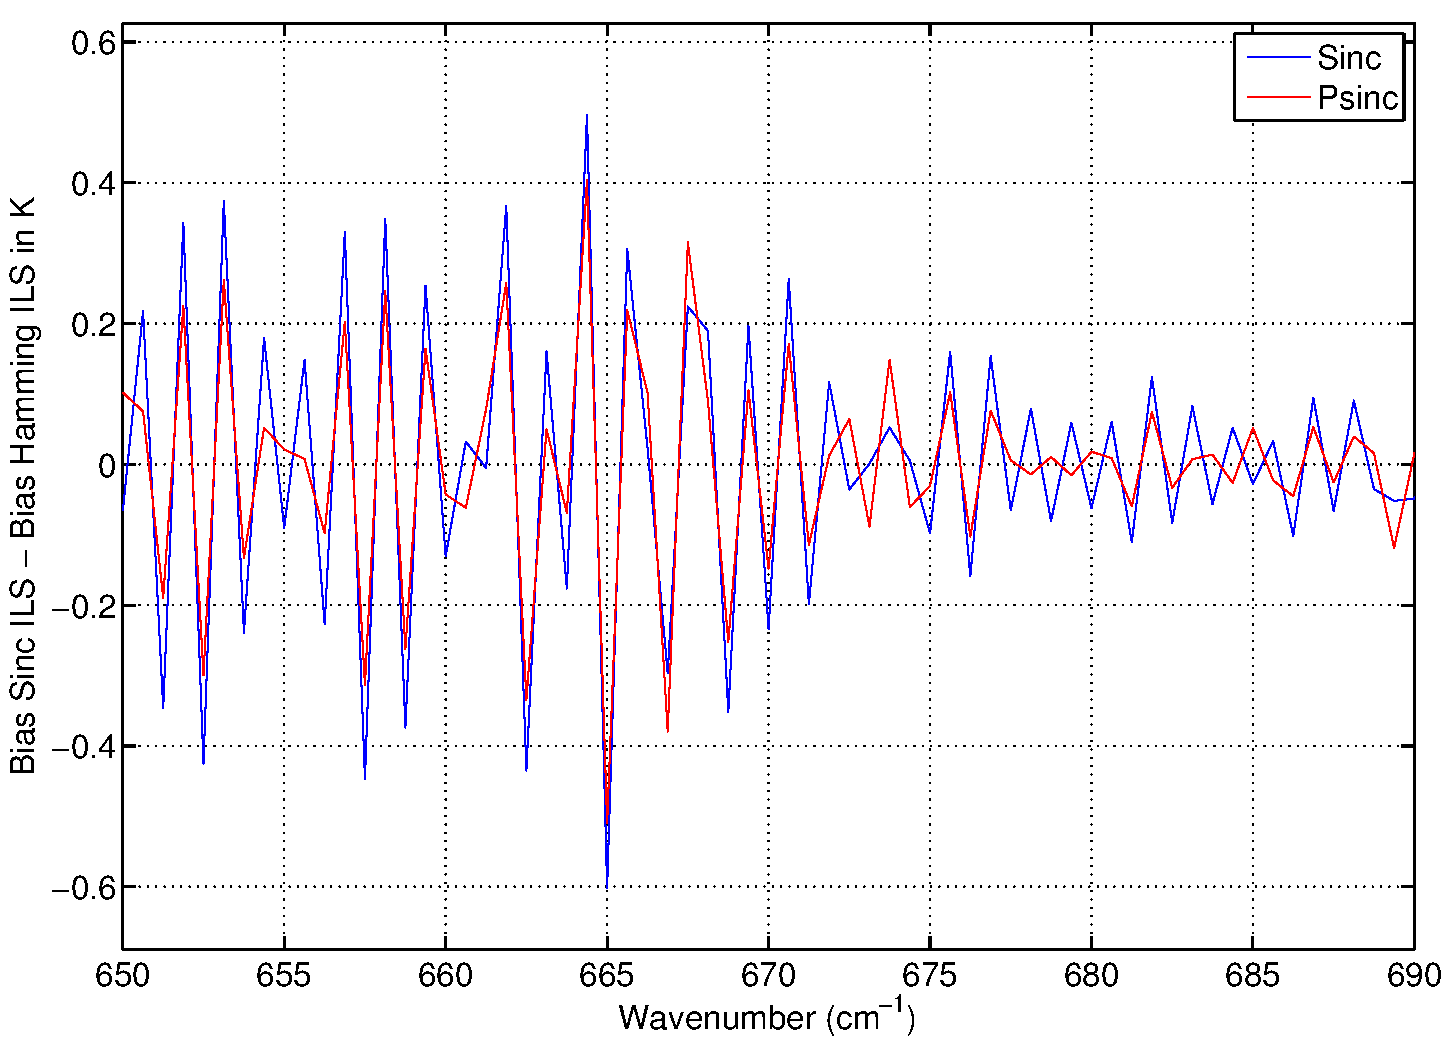
\includegraphics[scale=0.4]{strow_figs/bias_sinc_minus_bias_ham_LW.pdf}
\end{center}

LW zoom of $(\obs - \calc) - (H(\obs) - H(\calc))$ BT


\end{frame}
%----------- slide --------------------------------------------------%
\end{document}

